\chapter{Object-georiënteerd programmeren in Java}
In voorgaande cursussen is er al meer aandacht besteed aan 
object-georiënteerd programmeren in Java, maar het kan nooit kwaad 
om hier nogmaals het een en ander te herhalen. 

We gaan eerst kort in op Java en de Java Virtual Machine (JVM) om
vervolgens nader in te gaan op allerlei aspecten die je tegenkomt 
wanneer je in Java programmeert.

\section{Java}
Java is een veelgebruikte programmeertaal
waarmee allerlei verschillende soorten applicaties kunnen
worden gemaakt. De taal is in 1995 uitgebracht en is oorspronkelijk
ontworpen door James Gosling bij Sun Microsystems (later overgenomen door
Oracle). 

De kracht van Java zit hem in de JVM, 
een manier om Java (en andere programmeertalen die JVM-compatible zijn) 
te kunnen uitvoeren op verschillende soorten apparaten.

\section{De Java Virtual Machine (JVM)}
De CPU (\textit{Central Processing Unit} of \textit{processor}) 
in onze computer kan alleen machinecode lezen 
die hoort bij de betreffende CPU-architectuur.
Omdat machinecode lastig is te lezen, schrijven en organiseren
voor mensen, zijn er hogere programmeertalen 
uitgevonden (\textit{high-level languages}). 
Dit zijn talen die in meer of mindere mate verder verwijderd zijn van 
de concrete hardware en dus op een hoger abstractie niveau werken.
Er zijn talen die relatief dicht op de hardware zitten (zoals C en C++)
en er zijn talen waarbij de gebruiker vrijwel geen besef hoeft te hebben 
van de onderliggende hardware (zoals Python en JavaScript).
Talen als Java en C# zitten er een beetje tussenin.

\subsection{Compilatie}
Er zijn programmeertalen die eerst door de gebruiker moeten worden 
omgezet om te kunnen uitgevoerd. Dit noemen we \textit{compilatie}.
Een \textit{compiler} leest broncode van de ene taal en zet het om naar code
in de andere taal. Vaak gaat het hier om omzetting van een hogere taal 
(zoals C of C++) naar een lagere taal (zoals een assembly-taal of machinecode).
Zie Figuur~\ref{fig:compiler}.
Compilers zijn vaak erg knap geprogrammeerd. Niet alleen ondersteunen ze 
veel CPU-architecturen als uitvoer, vaak worden er tijdens compilatie 
allerlei optimalisaties aangebracht om de code sneller te laten draaien.
Hierdoor duurt het compileren mogelijk wat langer, maar de eindgebruiker
heeft er later profijt van!

\begin{figure}[H]
    \centering
    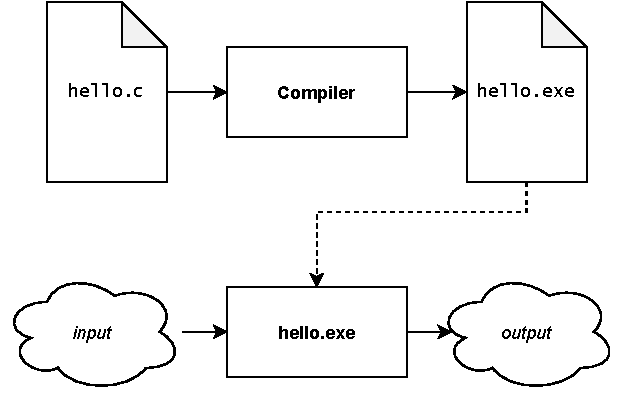
\includegraphics[width=.7\linewidth]{compilation}
    \caption{Compilatie, versimpeld weergegeven.}
    \label{fig:compiler}
    \index{compiler}
\end{figure}

Vaak moet de programmeur op de een of andere manier aan de compiler duidelijk 
maken welke bestanden allemaal samen moeten worden gevoegd in het uitvoerbestand.
Het kan soms een hele klus zijn om compilers met de hand in te stellen, 
hiervoor kunnen \textit{build tools} en 
\textit{integrated development environments (IDEs)}
uitkomst bieden. Dit soort tools zorgen ervoor dat programmeurs 
makkerlijker met de broncode kunnen werken.

\subsection{Interpretatie}
Een andere aanpak om hogere talen om te zetten naar machinetaal is door 
gebruik te maken van een \textit{interpreter}. Dit is een programma dat 
de hogere taal inleest en het rechtstreeks omzet naar uitvoering op de 
CPU. Zie Figuur~\ref{fig:interpreter}. Dit heeft als voordeel dat er geen compilatiestap meer nodig is, 
maar als nadeel dat er minder tussentijdse optimalisaties uitgevoerd worden.

\begin{figure}[H]
    \centering
    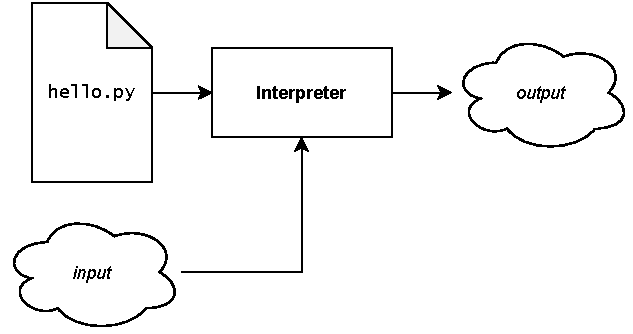
\includegraphics[width=.7\linewidth]{interpretation}
    \caption{Interpretatie, versimpeld weergegeven.}
    \label{fig:interpreter}
    \index{interpreter}
\end{figure}

Python en JavaScript zijn voorbeelden van geïnterpreteerde talen. Web browsers
hebben een ingebouwde JavaScript-interpreter om gebruikersinteractie te verwezelijken.

\subsection{Tussentalen}
Hogere programmeertalen zijn wat syntax en grammatica betreft vaak 
erg complex. Daarnaast compilers en interpreters veel CPU-architecturen 
ondersteunen met elk een eigen soort machinecode als uitvoerformaat.
Om deze complexiteit op te splitsen in beheersbare onderdelen, 
werken sommige talen met een soort "algemene" tussentaal. Deze algemene,
simpelere tussentaal wordt dan uitgelezen door een soort interpreter 
die dit weet uit te voeren voor verschillende CPU-architecturen.
Dit soort talen werken dus met een combinatie van een compiler en 
een interpreter, zie Figuur~\ref{fig:tussentaal}.

\begin{figure}[H]
    \centering
    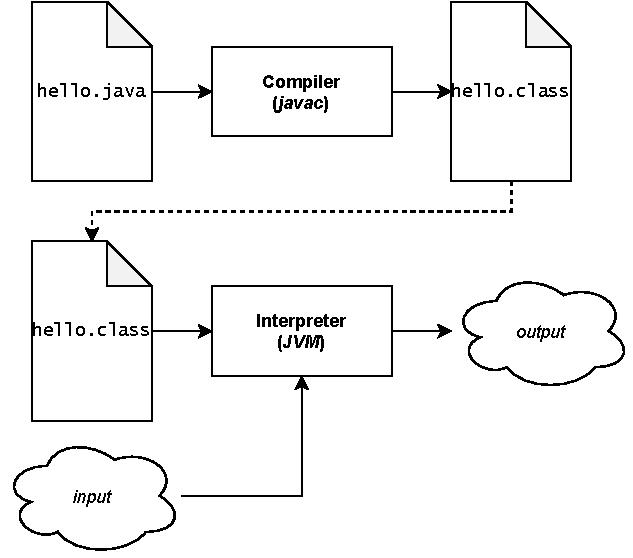
\includegraphics[width=.7\linewidth]{tussentaal}
    \caption{Tussentaal, versimpeld weergegeven.}
    \label{fig:tussentaal}
    \index{tussentaal}
\end{figure}

Java is een voorbeeld van een taal waarvan 
de broncode (\textit{Java-code}) eerst wordt 
omgezet in een tussentaal (\textit{bytecode}),
welke vervolgens wordt uitgevoerd door de \textit{Java Virtual Machine (JVM)}.
Nieuwere talen zoals \textit{Kotlin}, \textit{Clojure} en \textit{Scala} 
compileren ook naar bytecode en zijn dus ook uitvoerbaar door de JVM!

Een ander voorbeeld van een taal die met een tussentaal werkt is C\#.
Daarin wordt C\#-code eerst omgezet naar een 
\textit{intermediate representation (IR)} om vervolgens te worden uitgevoerd
door de \textit{Common Language Runtime (CLR)}.

\section{Typesysteem}
Voor een CPU is alle data binair: het bestaat uit enen en nullen.
In werkelijkheid zit er betekenis achter deze bits. 
De ene keer gaat het om een heel getal, de andere keer om een kommagetal
en weer een andere keer om een tekst of een lijst van getallen.

In een hogere programmeertaal maken we dit onderscheid middels \textit{data types}.
Het data type bepaalt wat je allemaal met een stuk data kunt doen en in hoeverre het 
compatibel is met een ander data type.

\subsection{Sterk en statisch getypeerd}
Er zijn programmeertalen die heel vergevingsgezind zijn ten aanzien van de types
die de programmeur gebruikt. Sommige talen, zoals Python, converteren waar mogelijk 
stilzwijgend data van het ene type naar dat van een ander type. Dat zie je veel 
in \textit{zwak getypeerde} talen.
Java is niet zo'n taal, maar is \textit{sterk getypeerd}. 
Dit houdt in dat de programmeur zijn datatypes nadrukkelijk moet aangeven
en de compiler klopt of de juiste types worden gebruikt. Hoewel dit erg 
wennen is als je nog wat minder bekend bent met de verschillende types,
voorkomt dit een aantal programmeerfouten en kan de compiler gemakkelijker
bepaalde optimalisaties uitvoeren.

In Java wordt \textit{type checking} in de compiler uitgevoerd. Er wordt 
puur op basis van de broncode gekeken of de gedeclareerde types en de beschreven 
operaties kloppen. Wanneer de types voor de compiler moeten worden aangegeven in 
een programmeertaal, noem je deze taal \textit{statisch getypeerd}. Talen waarin 
je het typesysteem vooral tijdens runtime tegenkomt (dus na compileren, bij uitvoering) 
zijn \textit{dynamisch getypeerde} talen als JavaScript en Python.

\subsection{Value types versus reference types}
In Java kennen we \textit{value types} en \textit{reference types}.
Value types zijn types die in het geheugen worden opgeslagen (in de \textit{stack}) 
op basis van hun waarde. 
Zo staat de integer 42 altijd op dezelfde plek in het geheugen voor een bepaalde 
methode-aanroep, onafhankelijk van welke variabele ernaar wijst. 

Reference types worden in het geheugen opgeslagen (in de \textit{heap}) 
op basis van hun instantie, hun identiteit.
Twee objecten worden op verschillende geheugenadressen opgeslagen, zelfs als hun 
waarden hetzelfde zijn!

Anders dan in bijvoorbeeld C++ wordt er in Java geen onderscheid gemaakt naar 
\textit{pass-by-value} of \textit{pass-by-reference}. We hoeven dus geen rekening 
te houden met pointer-logica. Alle method calls in Java werken 
volgens het principe van \textit{pass-by-value}, ook wanneer er een reference
type wordt meegegeven. De reference wordt dan als waarde meegegeven middels een
parameter. Je kan de reference zelf niet aanpassen, slechts de waarden waarnaar 
wordt gerefereerd. Je kan bijvoorbeeld een referentie naar een object meegeven 
als een parameter van een methode. 
Dat object kan je aanpassen via die referentie -- mits de publieke methodes dat toelaten binnen 
de methode. Je kan er niet voor zorgen dat er ineens een ander object op dezelfde plek in 
het geheugen komt. Dit kan in sommige andere talen wel, 
waar het voor enige verwarring kan zorgen onder developers.

\subsection{Primitive types}
\textit{Primitive types} zijn basale standaardtypen die door Java worden geboden.
Er zijn 8 verschillende primitive types in Java.
Zie Tabel~\ref{table:primitive-types}. 

\begin{table}[H]
    \centering
    \begin{tabularx}{\textwidth}{
        |>{\raggedright}l|>{\raggedright}X|>{\raggedright\arraybackslash}X|
    }
    \hline
    \textbf{Type} & \textbf{Betekenis} & \textbf{Voorbeeld} \\ \hline
        \textit{boolean}
        & een binaire waarheidswaarde van \texttt{true} of \texttt{false}
        & \texttt{boolean isGood = true;} \\ \hline
        \textit{byte}
        & een geheel getal met een grootte van 8 bits \newline 
        (van \(-128\, (-2^7)\) t/m \(127\, (2^7 - 1)\))
        & \texttt{// Base 10: 5} \newline \texttt{byte bits = 0b101;} \\ \hline
        \textit{short}
        & een geheel getal met een grootte van 16 bits \newline
        (van \(-32.768\, (-2^{15})\) t/m \(32.767\, (2^{15} - 1)\))
        & \texttt{short smallNumber = 1021;} \\ \hline
        \textit{integer}
        & een geheel getal met een grootte van 32 bits \newline
        (van \(-2.147.483.648\, (-2^{31})\) t/m \(2.147.483.647\, (2^{31} - 1)\))
        & \texttt{int largeNumber = 2312121;} \\ \hline
        \textit{long}
        & een geheel getal met een grootte van 64 bits \newline
        (van \(-2^{63}\) t/m \(2^{63} - 1\))
        & \texttt{long largerNumber = 323121211L;} \\ \hline
        \textit{float}
        & een komma-getal met een grootte van 32 bits \newline
        (van \(-2^{31}\) t/m \(2^{31} - 1\))
        & \texttt{float pi = 3.14F;} \\ \hline
        \textit{double}
        & een komma-getal met een grootte van 64 bits \newline
        (van \(-2^{31}\) t/m \(2^{31} - 1\))
        & \texttt{double pi = 3.1415D;} \\ \hline
        \textit{char}
        & een tekstteken met een grootte van 16 bits
        & \texttt{char letterX = `X`;} \\ \hline
    \end{tabularx}
    \caption{Java's primitive types}
    \label{table:primitive-types}
    \centering
\end{table}

Primitive types zijn value types, ze zijn dus ook immutable. Je kan ze wel 
overschrijven, maar niet (gedeeltelijk) aanpassen. 
In Java kunnen primitive types aangegeven worden met een kleine letter of een 
grote letter. Met een kleine letter (bijvoorbeeld \texttt{int}) 
verwijs je naar een \textit{unboxed type}. 
Dit zijn rauwe types zonder methodes; het zijn geen objecten.
Begint het type met een hoofdletter (bijvoorbeeld \texttt{Integer}), d
an is het een \textit{boxed type} en 
gedraagt het zich wel als een object. De JVM zorgt op veel plekken voor 
autoboxing. Dat betekent dat het op veel plekken niet zoveel uitmaakt of je 
verwijst naar de boxed of de unboxed variant. 

Wil je een methode aanroepen op 
een object, maar gaat het om de unboxed variant? Dan kan je het eerst omzetten 
door de waarde aan de constructor mee te geven. In de praktijk is het handig om 
zoveel mogelijk boxed types te gebruiken.

\subsection{Strings}
Strings zijn bedoeld om reeksen van teksttekens aan te geven.
Een string is geen primitive type in Java. Je kan er dus alleen 
naar verwijzen via \texttt{String}, een object van het type String. 
Omdat ze zoveel voorkomend zijn hebben ze een bijzonder karakter in Java. 
Zo kan je met een \textit{string literal} een String aanmaken:
\texttt{String text = "Hello world!"}. 

Net als primitive types zijn Strings ontworpen met het idee van 
immutability. Dat wil zeggen dat, hoewel het reference types zijn, hun waarde 
niet deels kunnen worden aangepast. Deze kan slechts in zijn geheel worden 
overschreven.

\section{Objecten en klassen}
Java is ontworpen met het idee van object-oriëntatie:
objecten zijn de centrale abstracties waarmee we ons werk doen.
Dit leidt tot een aantal voordelen, maar vereist ook wat denkwerk
bij het ontwerpen en realiseren van objecten. Hierover in een ander hoofdstuk meer.

We duiken in een aantal van Java's belangrijkste object-georiënteerde mogelijkheden
aan de hand van het domein van tweedimensionale geometrische vormen, zie Figuur~\ref{fig:shapes}.
\begin{figure}[H]
    \centering
    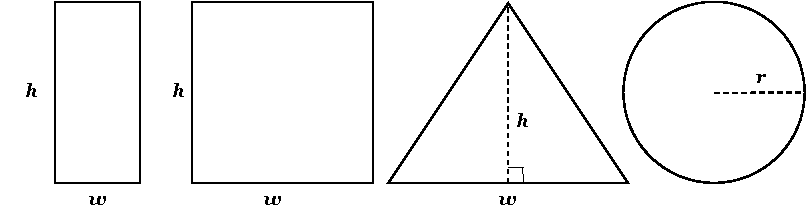
\includegraphics[width=.7\linewidth]{shapes}
    \caption{Geometrische vormen en hun dimensies.}
    \label{fig:shapes}
\end{figure}

Java is een \emph{klasse-gebaseerde} object-georiënteerde programmeertaal.
Dit betekent dat de programmeur nieuwe objecten kan definiëren door hiervoor 
nieuwe klassen aan te maken. Een klasse (\textit{class}) is een soort 
blauwdruk van een object en bepaalt het type van het object.
Zie bijvoorbeeld de \texttt{Rectangle}-klasse die ten grondslag kan 
liggen aan verschillende rechthoek-instanties met verschillende configuraties.
Zie Voorbeeld~\ref{code:rectangle}.

\begin{listing}[H]
\begin{minted}[linenos]{java}
public class Rectangle implements Shape2D {
    private Integer height;
    private Integer width;

    public Rectangle(Integer height, Integer width) {
        this.height = height;
        this.width = width;
    }

    public Double calculateArea() {
        return (double) (this.height * this.width);
    }

    public Boolean isLargerThan(Shape2D other) {
        return this.calculateArea() > other.calculateArea();
    }
}
\end{minted}
\caption{Een klasse voor een rechthoek.}
\label{code:rectangle}
\end{listing}

In \ref{code:rectangle} zien we dat \texttt{Rectangle} een klasse is
die een interface implementeert met de naam \texttt{Shape2D} 
(een tweedimensionale geometrische vorm). De klasse heeft 
dus het type \texttt{Rectangle} en als supertype \texttt{Shape2D}. Dit betekent 
dat we een object-instantie van het type \texttt{Rectangle} kunnen invullen 
waar om een \texttt{Shape2D} wordt gevraagd. Dat is een voorbeeld van polymorfisme.
Over interfaces en polymorfisme later meer, maar het is van belang om in te zien dat 
we verschillende implementaties kunnen maken van \texttt{Shape2D}. Zie Figuur~\ref{fig:uml-shapes}.

\begin{figure}[H]
    \centering
    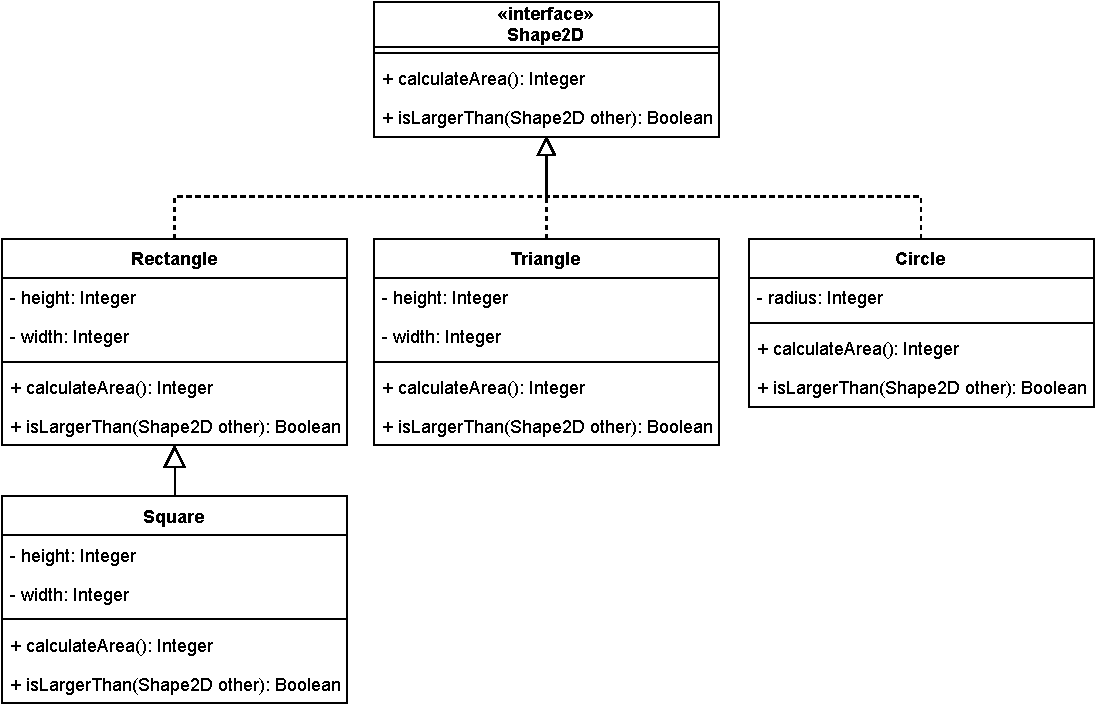
\includegraphics[width=.9\linewidth]{uml-shapes}
    \caption{Een UML klassendiagram van de verschillende shapes, inclusief realisatie en overerving.}
    \label{fig:uml-shapes}
\end{figure}

Objecten brengen toestand (\textit{fields}) en gedrag (\textit{methods}) onder 
in één eenheid, waarmee we kunnen praten via publieke methodes. 
Op die manier verbergt het object de interne complexiteit en wordt het onmogelijk
om van buiten het object afhankelijk te worden van hoe het object intern te werk gaat:
de implementatiedetails zijn verborgen.

\subsection{Fields}
De toestand van een object wordt bijgehouden in \textit{fields}
(velden, soms ook: \textit{attributes} of \textit{properties}).
In Voorbeeld~\ref{code:rectangle} kan je zien dat de fields zijn opgenomen in regels
2 en 3, namelijk de width (breedte) en height (hoogte), beide van het type Integer.

Het declareren van fields doen we vaak bovenin de klasse. Meestal beschrijf je een 
aantal modifiers (zie hierna), het type van de field en vervolgens 
de naam van het field. Het is belangrijk om een leesbare, menselijke naam te gebruiken 
die past bij het domein van ons systeem. 

We kunnen binnen een objectinstantie toegang krijgen tot 
een field door ernaar te verwijzen via \texttt{this}, bijvoorbeeld: \texttt{this.width}.

\subsection{Methods}
Met \textit{methods} (methodes) kunnen we gedrag toekennen aan een object.
We declareren een methode door deze in een klasse op te nemen. Een dergelijke 
declaratie (een \textit{method signature}) heeft de volgende onderdelen:
\begin{enumerate}
    \item \textit{modifiers}: geven bijzonderheden van de methode aan, 
    zoals bijvoorbeeld de zichtbaarheid vanuit andere klassen (zie hierna)
    \item \textit{return-type}: geeft aan wat voor een type er terug wordt gegeven 
    na het aanroepen van de methode
    \item \textit{parameter-types en -namen}: als er parameters zijn, 
    geef je deze aan met een type en een naam (zie: Voorbeeld~\ref{code:rectangle}, regels 14-16)
    \item \textit{checked exceptions die gegooid kunnen worden}: 
    als er checked exceptions (fouten die afgehandeld moeten worden) gegooid kunnen worden
    die niet in de methode worden afgehandeld, dien je deze te specificeren door \texttt{throws} 
    met daarachter de te gooien exception types
\end{enumerate}

Een voorbeeld is te vinden in Voorbeeld~\ref{code:rectangle}, regels 10-12 en regels 14-16.
Op deze manier hebben we de mogelijkheid toegevoegd om van een bestaande rechthoek
de oppervlakte te berekenen en de grootte te vergelijken met een ander tweedimensionale vorm.

Merk trouwens op dat we de oppervlakte omzetten van een integer naar een double. Dat doen we met de 
\textit{type cast} \texttt{(double)}. Java past hier autoboxing toe door de uiteindelijke
\texttt{double} automatisch om te zetten naar de in de return type aangegeven \texttt{Double}.

Methodes zijn, zoals je ziet, een krachtige manier om betekenis toe te voegen aan een project:
door de namen en typen van klassen en velden te lezen zien we met welke data we te maken hebben,
door de namen, return-typen en parameter-typen van methodes te lezen zien we wat we allemaal 
met een object kunnen doen.

Vaak kunnen we methods onderscheiden in \textit{queries}, die een waarde teruggeven
zonder iets aan te passen of een (externe) actie uit te voeren, en 
\textit{commands}, die iets aanpassen of iets anders doen en niet per se een 
waarde hoeven terug te geven. Het type \texttt{void} is gelijkwaardig aan \texttt{null}
(de afwezigheid van een waarde), maar geeft aan dat er geen intentie is dat de methode 
iets teruggeeft. Een query kan per definitie geen void als return type hebben. Er kan wel 
\texttt{null} terugkomen, wat aangeeft dat er geen waarde `gevonden' kon worden. 
In plaats van null is het overigens het overwegen waard om Optional te gebruiken.

We roepen een methode aan op een objectinstantie door tussen de instantie en de methode 
een punt te zetten en er haakjes achter te zetten. Moeten we argumenten meegeven voor 
de parameters, dan vullen we deze in de haakjes in. Zie Voorbeeld~\ref{code:method-call},
regel 4.

\begin{listing}[H]
\begin{minted}[linenos]{java}
Shape2D rectangleA = new Rectangle(10, 20);
Shape2D rectangleB = new Rectangle(20, 30);

if (rectangleB.isLargerThan(rectangleA)) {
    System.out.println("B is larger than A");
}

\end{minted}
\caption{We maken twee rechthoeken aan en kijken 
of rechthoek B groter is dan rechthoek A.}
\label{code:method-call}
\end{listing}

\subsubsection{Constructor}
In Voorbeeld~\ref{code:rectangle}, regels 5-7, zien we de constructor
van onze rechthoek. Het is een bijzonder soort methode die een objectinstantie
van een klasse maakt. We zien in Voorbeeld~\ref{code:method-call}, regels 1 en 2,
hoe we zo'n constructor in een andere klasse kunnen aanroepen. We kennen de instantie 
toe aan een variabele. Deze wijst nu naar een plekje in het geheugen waar de 
\texttt{Rectangle}-instantie is opgeslagen tijdens de duur van de applicatie.

Merk op dat we bij het declareren van de variabele het supertype hebben aangegeven.
Op deze manier zouden we ook de constructor van een andere klasse kunnen aanroepen 
en aan de variabele toekennen, mits deze ook \texttt{Shape2D} implementeert.

Onze IDE kan op basis van de aanwezige fields gemakkelijk een constructor genereren.
In IntelliJ kan je hiervoor op Windows en Linux de hotkeys \texttt{Alt + Insert} gebruiken, 
op MacOS \texttt{Command + N}.

\subsubsection{Getters en setters}
Op dit moment zijn de enige waardes die we uit ons object kunnen krijgen 
de oppervlakte (omgezet naar een double) en of het object groter is dan een ander object (Boolean).
De hoogte en breedte van een rechthoek kunnen we niet uit de objectinstantie opvragen.

Hoewel we hiermee voorzichtig moeten zijn omdat we zo koppeling op de 
implementatiedetails van het object mogelijk maken, kunnen we getters 
(of: \textit{accessors}) toevoegen 
om bij verborgen (\textit{private}) fields te kunnen.

Ook kunnen we de Rectangle van buitenaf niet aanpassen, als we eenmaal een instantie.
Een beetje zoals een \textit{value type}, moeten we een nieuwe Rectangle maken 
als we deze willen 'aanpassen'. Dit maakt code over het algemeen een stuk makkelijker 
te begrijpen (en en te parallelliseren). Vinden we dit wat minder belangrijk
(en vinden we koppeling op de interne toestand toelaatbaar), dan kunnen we 
ervoor kiezen om setters (ook: \textit{mutators}) toe te voegen. 
Zie Voorbeeld~\ref{code:accessors}.

\begin{listing}[ht]
\begin{minted}[linenos]{java}
public class Rectangle implements Shape2D {
    private Integer height;
    private Integer width;

    public Rectangle(Integer height, Integer width) {
        this.height = height;
        this.width = width;
    }

    // Other methods...

    public Integer getHeight() {
        return this.height;
    }

    public Integer getWidth() {
        return this.width;
    }

    public void setHeight(Integer height) {
        this.height = height;
    }

    public void setWidth(Integer width) {
        this.width = width;
    }
}
\end{minted}
\caption{Met getters kunnen we toegang krijgen tot fields en met setters kunnen we ze wijzigen.
Omdat de interne toestand niet meer is afgeschermd, 
brengt dit wel risico's mee ten aanzien van koppeling.}
\label{code:getters-setters}
\end{listing}

Ook dit is eenvoudig te genereren door je IDE op basis van de aanwezige fields.
In IntelliJ kan je hiervoor op Windows en Linux de hotkeys \texttt{Alt + Insert} gebruiken, 
op MacOS \texttt{Command + N}.

\subsubsection{Gelijkwaardigheid: \texttt{equals()} en \texttt{hashCode()}}
Omdat objecten reference types zijn, wordt de \texttt{equals}-methode standaard gebaseerd 
op het geheugenadres van de instanties. Alleen als deze gelijk zijn is sprake van 
hetzelfde object, zie Voorbeeld~\ref{code:identity-equality}.

\begin{listing}[H]
\begin{minted}[linenos]{java}
Shape2D rectangleC = new Rectangle(20, 30);
Shape2D rectangleD = new Rectangle(20, 30);

// Prints: false
System.out.println(rectangleC.equals(rectangleD));

Set<Shape2D> shapes = new HashSet<>();
shapes.add(rectangleC);

// Prints: false
System.out.println(shapes.has(rectangleD));

\end{minted}
\caption{Standaard \texttt{equals}- en \texttt{hashCode}-methodes: 
gelijkwaardigheid op basis van identiteit.}
\label{code:identity-equality}
\end{listing}

Dit is niet altijd wat we willen. Soms willen we gelijkwaardigheid
vaststellen op basis van waardes, in plaats van identiteit. Daarvoor kunnen we 
de \texttt{equals}-methode overschrijven.

De \texttt{hashCode}-methode is vergelijkbaar, maar ziet op hoe objecten 
efficient kunnen worden bewaard in 
een \texttt{HashMap}, \texttt{HashSet} of \texttt{HashTable}.
Normaliter wordt dat ook op basis van geheugenadres gedaan. Ook dat is te overschrijven.

\begin{listing}[H]
\begin{minted}[linenos]{java}
public class Rectangle implements Shape2D {
    private Integer height;
    private Integer width;

    // Constructor + other methods...

    @Override
    public boolean equals(Object o) {
        if (this == o) return true;
        if (o == null || getClass() != o.getClass()) return false;
        Rectangle rectangle = (Rectangle) o;
        return Objects.equals(height, rectangle.height) 
            && Objects.equals(width, rectangle.width);
    }

    @Override
    public int hashCode() {
        return Objects.hash(height, width);
    }
}
\end{minted}
\caption{Door IDE gegenereerde \texttt{equals}- en \texttt{hashCode}-methodes.}
\label{code:hashcode-equals}
\end{listing}

Beide methodes zijn te genereren door onze IDE, zie Voorbeeld~\ref{code:hashcode-equals}
Je zult zien dat onze IDE zelfs een aantal randgevallen afdekt in de \texttt{equals}-methode!
In IntelliJ kan je hiervoor op Windows en Linux wederom 
de hotkeys \texttt{Alt + Insert} gebruiken, op MacOS \texttt{Command + N}.
Na deze toevoegingen printen beide gevallen uit Voorbeeld~\ref{code:identity-equality}
\texttt{true}!

\subsection{Inheritance}
Inheritance (\textit{overerving}) is een veelgebruikt maar controversieel mechanisme in Java 
om aan te geven dat een subklasse (ook: \textit{child}) is afgeleid van 
een superklasse (ook: \textit{parent}) en dat deze subklasse  
fields en methods overneemt van deze superklasse.

Dit is te zien in Voorbeeld~\ref{code:inheritance}. Een vierkant is een 
specifiek soort rechthoek, namelijk een rechthoek met gelijke zijden.
Daarom roepen we in de constructor van Square de constructor aan van 
de superklasse, Rectangle, middels de \texttt{super}-methode en we vullen 
de size voor zowel de height als de width in.

\begin{listing}[H]
\begin{minted}[linenos]{java}
public class Square extends Rectangle {
    public Square(Integer size) {
        super(size, size);
    }
}
\end{minted}
\caption{Een Square is een specifiek soort Rectangle.}
\label{code:inheritance}
\end{listing}

Wanneer we een Square-instantie hebben kunnen we daarop dezelfde 
niet-private methodes aanroepen als die op Rectangle zijn gedeclareerd.
Dan kan onze Square-klasse zo klein blijven!
Merk op dat een Square ook de Shape2D interface implementeert 
-- namelijk via diens superklasse.

\subsubsection{Interface inheritance versus implementation inheritance}
Soms beschouwt men het implementeren van een interface
als een onderdeel van inheritance. Wanneer men specifiek 
die vorm van overerving bedoelt, spreekt men van \textit{interface inheritance}
of \textit{realisatie}.

\textit{Implementation inheritance} is de meer klassieke vorm van overerving.
Implementation inheritance wordt veel gebruikt om bepaalde stukken code gemakkelijk te delen tussen klassen,
maar daarin zit gelijk ook het gevaar: je koppelt de super- en subklassen aan elkaar.
Wanneer een superklasse meerdere subklassen heeft, ontstaat het gevaar dat subklassen indirect 
aan elkaar gekoppeld raken. Veranderingen in een superklasse ten behoeve van één subklasse 
komen al gauw terecht in alle subklassen. Dit kan een risico vormen voor de onderhoudbaarheid.
Probeer implementation inheritance zoveel mogelijk te beperken tot gevallen van ware inheritance 
of slechts tot het overerven van een \textit{abstracte} klasse (zie hierna).

Het is in Java niet mogelijk dat een klasse van meerdere klassen overerft, 
terwijl het wel mogelijk is dat een klasse meerdere interfaces implementeert.

\subsection{Modifiers}
In de declaratie van fields en methodes kunnen we met behulp van keywords modifiers toevoegen.
Er zijn verschillende modifiers beschikbaar in Java, wij behandelen de belangrijkste. 

\subsubsection{Access modifiers: \texttt{public}, \texttt{protected} en \texttt{private}}
Met access modifiers (of \textit{visibility modifiers}) kunnen we 
beperken welke andere klassen allemaal bij een bepaalde field of method kunnen komen.
Een \texttt{public} field of method is door elke klasse benaderbaar, 
een \texttt{private} field of method is enkel door de eigen klasse benaderbaar.
Daarnaast hebben we nog \texttt{protected}. Een field of method met die modifier 
is alleen niet benaderbaar door de buitenwereld, maar wel bijvoorbeeld door 
subklassen, door klassen binnen dezelfde package en de eigen klasse. 
Wanneer we geen modifier toevoegen, is er sprake van een \textit{package-private}
field of method: deze zijn alleen zichtbaar voor de eigen klasse en binnen
dezelfde package. Zie Tabel~\ref{table:access-modifiers}.

Klassen zelf kunnen ook als \texttt{public} (iedereen kan erbij) 
of \textit{package-private} (geen modifier; alleen iedereen binnen package kan erbij).

\begin{table}[H]
    \centering
    \begin{tabularx}{\textwidth}{
        |>{\raggedright}l|>{\raggedright}X|>{\raggedright}X|>{\raggedright}X|>{\raggedright\arraybackslash}X|
    }
    \hline
    \textbf{Access modifier} & \textbf{Class} & \textbf{Package} & \textbf{Subclass} & \textbf{Outside} \\ \hline
        \texttt{public} & Y & Y & Y & Y \\ \hline
        \texttt{protected} & Y & Y & Y & N \\ \hline
        \textit{(no modifier)} & Y & Y & N & N \\ \hline
        \texttt{private} & Y & N & N & N \\ \hline
    \end{tabularx}
    \caption{Java's access modifiers}
    \label{table:access-modifiers}
    \centering
\end{table}

Access modifiers zijn een erg krachtig wapen in de strijd tegen koppeling. 
Door gebruik te maken van 
strikte access modifiers kan je namelijk bepaalde zaken afschermen voor de buitenwereld, 
zodat er minder afhankelijkheid kan bestaan
op de interne implementatiedetails van een klasse.

\subsubsection{De \texttt{final}-modifier}
Met de \texttt{final}-modifier kan je ervoor zorgen dat 
een field of variabele binnen een methode niet opnieuw toegekend 
kan worden. 

Wanneer de \texttt{final}-modifier wordt gebruik voor een 
klasse-, field- of methodedeclaratie betekent dit ook dat deze niet 
overschreven kan worden door een subklasse.

Final kan als erg beperkend worden opgevat: velden kunnen niet makkelijk 
overschreven worden. Het voordeel daarvan is echter dat het gebruik van je code 
voorspelbaarder wordt omdat je er zeker van kan zijn dat iets niet wordt aangepast.
Daarom wordt soms aanbevolen om fields en klassen standaard 
final te maken en alleen final weg te halen wanneer je overschrijfbaarheid
en implementation inheritance wil toelaten. 
Als uitbreidbaarheid je doel is, is het vaak 
een goed idee om in plaats van implementation inheritance eerst  
naar een compositie-gebaseerde oplossing te zoeken.

\subsubsection{De \texttt{abstract}-modifier}
Met de \texttt{abstract}-modifier geef je aan dat de klasse of 
methode niet op zichzelf kan bestaan, maar moet worden ingevuld
door een subklasse. Vaak voeg je voor de naam van de abstracte klasse
het voorvoegsel \texttt{Base} toe.

Met de \texttt{abstract}-modifier móet je dus altijd een subklasse hebben
om het als abstract aangemerkte element in te vullen.
Je zal dan ook nooit een \texttt{abstract}-modifier combineren met 
een \texttt{final}-modifier voor dezelfde declaratie.

\subsubsection{De \texttt{static}-modifier}
Tot dusver hebben we methods en fields alleen maar gedeclareerd op 
\emph{objecten}, instanties.
We kunnen ook methodes maken die op de \emph{klasse} worden aangeroepen.
Er zijn namelijk fields die we in het algemeen willen kunnen bijhouden
of methods die we onafhankelijk van enige instantie willen aanroepen.
Daarvoor is de \texttt{static}-modifier uitgevonden.

Een typische reden om een static field te maken is voor
het declareren van een constante. Omdat een constante per definitie
niet gewijzigd hoort te worden, kunnen we de \texttt{static}-modifier combineren 
met de \texttt{final}-modifier. Zo kunnen we een klasse voorzien van een vaste waarde 
en het een duidelijke naam geven! 
Dit ziet er dan bijvoorbeeld uit, zoals in Voorbeeld~\ref{code:circle}.
In de praktijk is het overigens een beter idee om gebruik te maken van
de ingebouwde \texttt{Math.PI} constante.

\begin{listing}[H]
\begin{minted}[linenos]{java}
public class Circle implements Shape2D {
    private static final float PI = 3.14159265359f;

    private Integer radius;

    public Circle(Integer radius) {
        this.radius = radius;
    }

    public Double calculateArea() {
        return 2 * PI * this.radius;
    }

    public Boolean isLargerThan(Shape2D other) {
        return this.calculateArea() > other.calculateArea();
    }
}
\end{minted}
\caption{Een Circle-klasse met PI als static final methode.}
\label{code:circle}
\end{listing}

Static methods worden veel gebruikt in plaats van dat een klasse voorzien is van 
verschillende constructors voor verschillende creatie-wijzen.
In Java kan een methode vaker worden gedeclareerd met andere parameters, zo kan 
het gedrag variëren gebaseerd op het type van het argument dat aan een methode wordt meegegeven.
Dit noem je \textit{method overloading}. Het is echter vaak wenselijk om expliciet 
aan te geven wat je wil bereiken met een methode, zodat foutjes kunnen worden voorkomen.
Hiervoor zou je met behulp van static methods een \textit{named constructor} kunnen maken.

Stel dat we een Circle willen kunnen instantiëren op basis van een Rectangle, waarbij we 
de kortste zijde van het rechthoek pakken als straal (radius). Dan ziet dat eruit als 
in Voorbeeld~\ref{code:named-constructor}.

\begin{listing}[H]
\begin{minted}[linenos]{java}
public class Circle implements Shape2D {
    private static final float PI = 3.14159265359f;

    private Integer radius;

    public Circle(Integer radius) {
        this.radius = radius;
    }

    public static Circle fromRectangle(Rectangle rectangle) {
        Integer radius = rectangle.determineShortestSide();
        return new Circle(radius);
    }

   // Other methods...
}

// In Rectangle:
public class Rectangle implements Shape2D {
    // All other fields and methods ...
    
    public Integer determineShortestSide() {
        return Math.min(this.width, this.height);
    }
}
\end{minted}
\caption{Een named constructor: een statische methode die werkt als een constructor.}
\label{code:named-constructor}
\end{listing}

Merk op dat we in Rectangle de methode \texttt{determineShortestSide} hebben opgenomen,
waarin we de ingebouwde static method \texttt{Math.min} gebruiken om het minimum 
(de kleinste) van twee waarden te bepalen. 

Om een Circle aan te maken op basis van een Rectangle, roepen we de methode 
\texttt{fromRectangle} aan op de \emph{Circle-klasse} (niet een object-instantie).
\begin{listing}[H]
\begin{minted}[linenos]{java}
Shape2D rectangleE = new Rectangle(10, 20);
Shape2D circleA = Circle.fromRectangle(rectangleE);
\end{minted}
\caption{Het aanroepen van een named constructor als statische methode op de Circle-klasse.}
\label{code:named-constructor-invocation}
\end{listing}

\section{Enumerations (enums)}
Stel dat onze geometrische vormen voorzien kunnen worden van 
één van de volgende drie kleuren: \textit{red}, \textit{green}, \textit{blue}.
Hoe zouden we deze beperkte set aan mogelijkheden als field kunnen declareren?

Een eerste gedachte is misschien om met strings te werken de kleur te bepalen 
op basis van de waarde van de string. Maar wat doen we wanneer er sprake is van een
string die niet correct is gespeld of als iemand \textit{yellow} invult?
Het aantal mogelijke strings is oneindig. We zouden natuurlijk bij het invoeren 
een (runtime) check kunnen uitvoeren of de invoer klopt met de verwachte red, green of blue.

We zouden ook kunnen werken met drie booleans: isRed, isGreen en isBlue. 
Maar wat doen we als we een extra kleur willen ondersteunen in de toekomst?
En hoe zit het als we (per ongeluk) twee booleans true maken?

Het is moge duidelijk zijn: we hebben een oplossing nodig om een beperkte set
aan mogelijkheden te modelleren als een soort keuzemenu van constantes. 
De oplossing kan gevonden worden in enums. Een enum is in Java een speciaal soort 
klasse. Een enum draagt ook een type. 
We kunnen de enum aanmaken als onderdeel van een klasse of, overzichtelijk, in zijn eigen .java-bestand.
Zie Voorbeeld~\ref{code:enums}.

\begin{listing}[H]
\begin{minted}[linenos]{java}
public enum Color {
    RED,
    GREEN,
    BLUE
}
\end{minted}
\caption{Enums zijn handig om keuzemogelijkheden mee te modelleren.}
\label{code:enums}
\end{listing}

Stel nu dat we een Rectangle van een kleur willen voorzien, dan kunnen we 
de enum als een field opnemen en de keuzevrijheid bieden bij het instantiëren
van een object (het aanroepen van de constructor), zie Voorbeeld~\ref{code:enum-rectangle}.

\begin{listing}[H]
\begin{minted}[linenos]{java}
public class Rectangle implements Shape2D {
    private Integer height;
    private Integer width;
    private Color color;

    public Rectangle(Integer height, Integer width, Color color) {
        this.height = height;
        this.width = width;
        this.color = color;
    }
}

// Usage:
public class Main {
    public static void main(String[] args) {
        Shape2D redRectangle = new Rectangle(20, 10, Color.RED);
    }
}

\end{minted}
\caption{Je kunt naar het type van een enum verwijzen in de declaratie van een field, net zoals bij reguliere klassen.}
\label{code:enum-rectangle}
\end{listing}

Enums gebruik je om het aantal mogelijkheden te beperken. Het grote voordeel hiervan is dat je 
een minder strikt hoeft te valideren, zoals bij een string of een integer. Hier kan je IDE ook 
handig gebruik van maken. Deze kan een waarschuwing geven wanneer je in een switch-statement niet 
alle takken van een enum hebt afgedekt. Je kan zelfs alle takken automatisch laten genereren!

Een ander voordeel van enums is dat je kan loopen over de mogelijke waarden. Dit kan erg handig zijn 
als je alle permutaties ergens van wil weergeven.

\section{Interfaces}
Als we terugkijken naar Figuur~\ref{fig:uml-shapes} en de verschillende codevoorbeelden uit dit hoofdstuk,
zien we dat onze klassen de Shape2D-interface implementeren. Maar hoe ziet deze interface eruit?
Dit zien we in Voorbeeld~\ref{code:interface}.

\begin{listing}[H]
\begin{minted}[linenos]{java}
public interface Shape2D {
    Double calculateArea();
    Boolean isLargerThan(Shape2D other);
}
\end{minted}
\caption{Een interface legt vast welk gedrag implementaties moeten bieden.}
\label{code:interface}
\end{listing}

Via een interface kan je vastleggen welk gedrag je verwacht van een implementatie van
de interface. Sommige mensen vergelijken een interface een contract, maar het kan helpen 
om het eerder te zien als een soort wet. Een Shape2D is alleen geldig als het voorziet in 
het berekenen van de oppervlakte (en een Double teruggeeft) en als het kan bepalen of het 
groter is dan een andere Shape2D (en een Boolean teruggeeft).

Interfaces zijn van groot belang om flexibele software te bouwen, omdat je ermee afhankelijkheden 
kunt reguleren. Een interface biedt een soort garantie: als een klasse afhankelijk is van een 
Shape2D en deze wordt ingevuld met een Rectangle, dan kan deze altijd worden vervangen met een 
andere Shape2D. Op deze manier kan je dus ook nieuwe shapes ondersteunen zonder bestaande 
shapes aan te passen! Laten we bijvoorbeeld een Triangle maken. Zie Voorbeeld~\ref{code:triangle}.

\begin{listing}[H]
\begin{minted}[linenos]{java}
class Triangle implements Shape2D {
    private Integer height;
    private Integer width;

    public Triangle(Integer height, Integer width) {
        this.height = height;
        this.width = width;
    }

    public Double calculateArea() {
        return 0.5 * (this.height * this.width);
    }

    public Boolean isLargerThan(Shape2D other) {
        return this.calculateArea() > other.calculateArea();
    }
}
\end{minted}
\caption{Een Triangle is een Shape2D.}
\label{code:triangle}
\end{listing}

Een Java-klasse kan meerdere interface implementeren.

\section{Generics}
Wat nu als we een soort container type hebben, waarbij we 
ook het type willen kunnen variëren van de elementen in die container?
Dat is waar \textit{generics} voor zijn bedoeld: \textit{parameterized types}, 
hogere abstracties waarbij het type van de 
opgenomen elementen later kan worden ingevuld dankzij een \textit{type argument}.
Dit is een feature die sinds JDK 1.5 in Java is opgenomen.

\subsection{Collections}
Dit zie je veel bij verzamelingstypen (\textit{collections}), zoals een List, Set of Map.
Zie Figuur~\ref{fig:java-collections} voor een overzicht van allerlei klassen en interfaces
om verzamelingen te modelleren.

\begin{figure}[H]
    \centering
    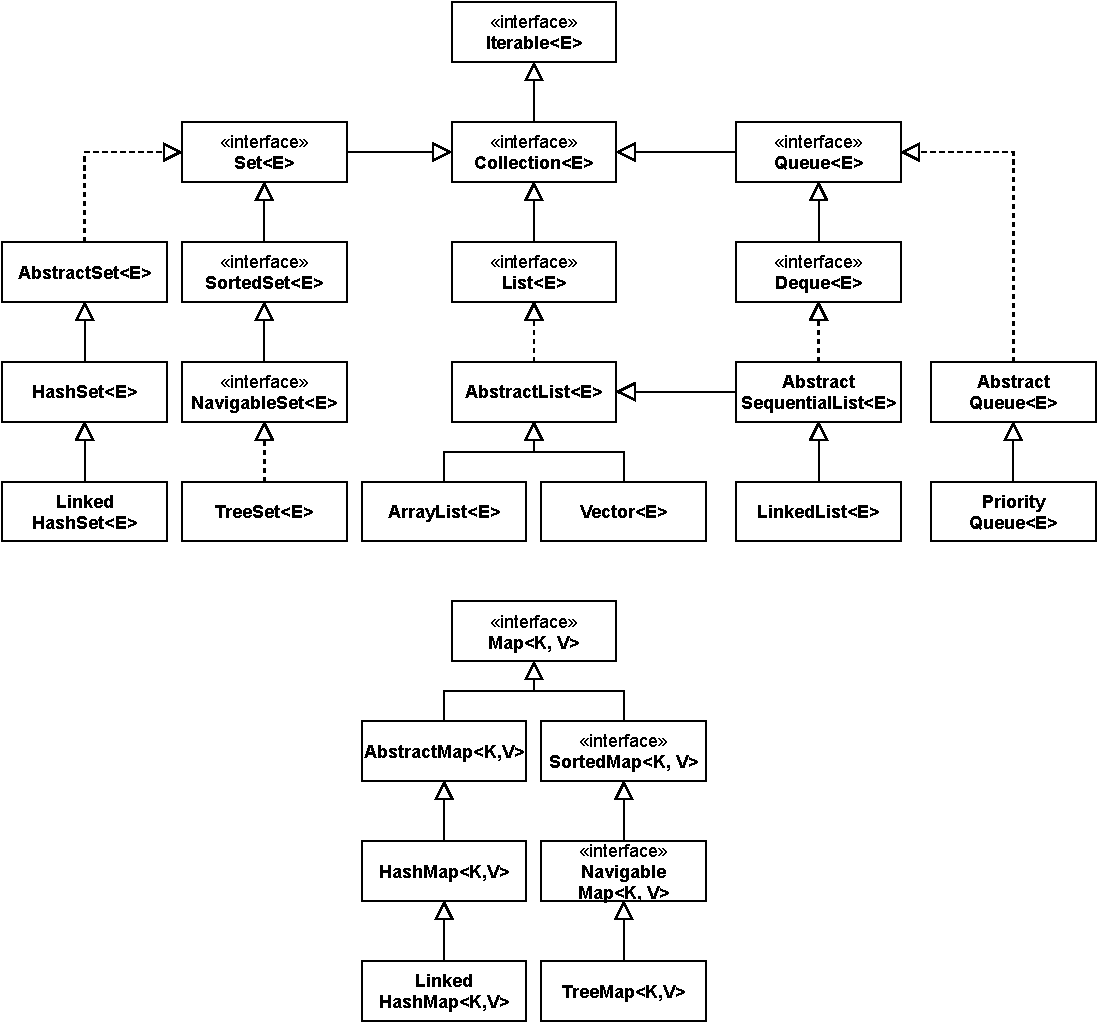
\includegraphics[width=.9\linewidth]{java-collections}
    \caption{Allerlei verschillende generic collection interfaces en classes van de Java Collections API.}
    \label{fig:java-collections}
\end{figure}

Elke soort collectie heeft zijn eigen doel. 
Om bijvoorbeeld een lijst van shapes aan te geven, 
kan je verwijzen naar \texttt{List<Shape2D>} (\textit{a list of shapes})
en deze invullen met een ArrayList<Shape2D> implementatie.
Waar lijsten echter vooral zijn bedoeld om elementen aan te bieden op een bepaalde volgorde,
gebruiken we sets vooral om bij te houden of we iets gezien hebben of niet. Een element 
kan maar één keer in een set zitten en een set bevat handige operaties om set logica 
uit te voeren. Een set van namen kan bijvoorbeeld weergegeven worden als 
\texttt{Set<Name>} (\textit{a set of names}).
Een map is bedoeld als een doorzoekbaar register (een dictionary),
waarbij een \textit{key} van een bepaald type kan verwijzen naar 
een \textit{value} van een bepaald ander type. Stel dat we bijvoorbeeld
willen bijhouden hoe vaak een bepaalde naam voorkomt in een groep,
dan kunnen we een \texttt{Map<Name, Integer>} (\textit{a map of names to integers})
bijhouden.

In dit geval zijn de List, Set en Map allemaal generic interfaces en
worden de type arguments ingevuld door Shape2D, Name en Integer.
Maar hoe definieer je een generic type? Laten we eens kijken naar de 
een deel van de Map-interface, zoals deze in Java is gedefinieerd,
zie Voorbeeld~\ref{code:map-generic}.

\begin{listing}[H]
\begin{minted}[linenos]{java}
public interface Map<K, V> {
    V put(K key, V value);
    V get(Object key);
    // Much more methods...
}
\end{minted}
\caption{Een deel van de generic Map-interface zoals deze is opgenomen in Java.}
\label{code:map-generic}
\end{listing}

In Voorbeeld~\ref{code:map-generic} zien we dat twee type arguments:
K en V. Deze types kunnen later worden ingevuld voor de elementen die 
als respectievelijk \textit{key} en \textit{value} worden opgenomen in de Map.
Je kan in een map dus een object van het ene type laten wijzen naar een 
object van het andere type 
(bijvoorbeeld een String naar een Integer, of een FullName naar een Address).

\subsection{Functional interfaces, streams, lambda expressions}
Sinds Java 8 kunnen we functies gebruiken als object. Dit zijn speciale objecten 
die een \textit{functional interface} implementeren. Je kan 
een functie declareren als variabele, teruggeven uit een methode of gebruiken 
als parameter. Dit maakt het makkelijker om bepaald gedrag mee te geven en 
te variëren aan een bestaande datastructuur. Dit klinkt nogal ingewikkeld en het 
is even wennen, maar je kan er een boel mee!

Een plek waar dit soort functies met name veel gebruikt worden is door een 
specifieke operatie uit te voeren op de elementen in een verzameling, bijvoorbeeld
het berekenen van de som van alle getallen in een lijst 
het aanpassen van alle waarden in een set of 
het filteren van bepaalde element uit een verzameling.
Hiervoor kan je sinds Java 8 gebruik maken van de \textit{Streams API}.
Op een verzameling in Java kan je \texttt{.stream()} aanroepen en vervolgens 
een methode die een functional interface verwacht. Een \texttt{Stream<T>} is 
een generiek type waarbij de elementen worden aangeboden als een reeks waarden over tijd.

Neem bijvoorbeeld een methode om uit een lijst van namen (\texttt{List<String>}),
de namen te verzamelen die beginnen met een bepaalde letter of reeks letters.
Met een for-loop zouden we dat bijvoorbeeld als volgt doen (Figuur~\ref{code:filter-loop}):

\begin{listing}[H]
\begin{minted}[linenos]{java}
public class FriendsList {
    private List<String> names = 
        List.of("Alex", "Bert", "Arnold", "Anton");

    public List<String> selectNamesByPrefix(String prefix) {
        List<String> selection = new ArrayList<>();

        for (String name : names) {
            String lowerCaseName = name.toLowerCase();
            if (lowerCaseName.startsWith(prefix)) {
                selection.add(name);
            }
        }

        return selection;
    }
}
\end{minted}
\caption{Het selecteren van namen op basis van een bepaalde prefix met behulp van een loop.}
\label{code:filter-loop}
\end{listing}

Als we gebruik maken van de Streams API ziet dezelfde method eruit als in Figuur~\ref{code:filter-streams}.

\begin{listing}[H]
\begin{minted}[linenos]{java}
public class FriendsList {
    private List<String> names = 
        List.of("Alex", "Bert", "Arnold", "Anton");

    public List<String> selectNamesByPrefix(String prefix) {
        return names.stream()
            .map(name -> name.toLowerCase())
            .filter(name -> name.startsWith(prefix))
            .collect(Collectors.toList());
    }
}
\end{minted}
\caption{Het selecteren van namen op basis van een bepaalde prefix met behulp van de Streams API.}
\label{code:filter-loop}
\end{listing}

Met \texttt{.stream()} veranderen we de lijst in een stream, zodat we er 
stream-operaties op kunnen uitvoeren.
Aan de \texttt{map} en \texttt{filter} methodes kunnen we een functie meegeven.
In het geval van de map-methode is het een functie die een String transformeert 
naar een andere String (\texttt{Function<String, String>}). In het geval 
van de filter-methode is geven we een predicate mee (\texttt{Predicate<String>}). 
Dit is een functie die een boolean teruggeeft op basis van een bepaalde invoer, in ons geval een String.
De filter-methode selecteert elementen op basis van de meegegeven predicate function.
Ten slotte moeten we de Stream weer omzetten naar een lijst, dat doen we met een \texttt{Collector}.

De pijlfunctie die we meegeven aan een stream-operatie noem je een \textit{lambda expressie} of \textit{arrow function}.
Dit een verkorte manier om een functie te declareren. De compiler check wel of het een verwachte en kloppende
implementatie oplevert van een functional interface.
Soms kan, in plaats van een lambda expressie, ook verwijzen naar een methode op een bepaalde instantie door naar diens naam 
op de klasse te wijzen. In het voorbeeld zouden we \texttt{name -> name.toLowerCase()} kunnen vervangen 
met \texttt{String::toLowerCase}.

Er zijn een boel verschillende stream-operaties en hoop verschillende soorten functional interfaces.
Het is ook mogelijk om zelf functional interfaces te declareren. Dat gaat te ver voor nu.

\subsection{Optionals}
In Java 8 is het generieke type van de \textit{Optional<T>} toegevoegd aan de taal.
De \texttt{T} is een \textit{type argument} dat door de developer zelf ingevuld kan worden.
Optionals zijn bedoeld als alternatief voor \texttt{null} en het voorkomen van 
\texttt{NullPointerException}s. Deze foutmelding krijg je bijvoorbeeld wanneer 
je een methode of veld op \texttt{null} probeert aan te roepen. Vaak gebeurt dit 
wanneer je uit een opslag iets probeert op te vragen dat er niet is. De standaardoplossing
hiervoor is om overal waar je \texttt{null} kan verwachten te checken of 
er sprake is van \texttt{null} of niet. Helaas kan onze compiler niet goed statisch (tijdens compilatie)
bepalen of we voldoende hebben gecheckt of we null terug kunnen krijgen.
Optional probeert daarbij te helpen en voegt daarnaast
wat methoden toe die de code simpeler kunnen maken.

Stel we hebben een methode die \texttt{Optional<User>} teruggeeft. Dan krijgen we 
een Optional-object terug, waarin een User \textit{kan} zitten. Dat hoeft niet zo 
te zijn. Door Optional als type te gebruiken (in plaats van \texttt{null} terug te geven),
kunnen compiler en IDE gemakkelijker waarschuwen als we vergeten om te checken of 
er wel daadwerkelijk een waarde terug wordt gegeven.

Het handige aan Optionals zijn de methodes die code een stukje simpeler kunnen maken.
Voor \texttt{Optional<User>} kunnen we de methodes aanroepen als in Tabel~\ref{table:optional-methods}.

\begin{table}[H]
    \centering
    \begin{tabularx}{\textwidth}{
        |>{\raggedright}l|>{\raggedright}X|>{\raggedright\arraybackslash}X|
    }
    \hline
    \textbf{Methode} 
    & \textbf{Return type} 
    & \textbf{Beschrijving} 
    \\ \hline
        
    \texttt{isPresent}
    & \texttt{boolean}
    & Geeft terug of er een waarde in de optional zit of niet.
    \\ \hline

    \texttt{ifPresent}
    & \texttt{void}
    & Voert de meegeven \textit{consumer function} uit als er een waarde inzit, maar 
    doet niets als deze leeg is.
    \\ \hline

    \texttt{orElse}
    & \texttt{User}
    & Geeft de ingesloten User terug of de aangegeven default User als de optional leeg is.
    \\ \hline

    \texttt{orElseThrow}
    & \texttt{User}
    & Geeft de ingesloten User terug of gooit een exception als de optional leeg is.
    \\ \hline

    \texttt{get}
    & \texttt{User} (gooit een \texttt{NoSuchElementException} als leeg)
    & Met deze methode kan je de waarde uit de Optional halen. 
    Dit kan je eigenlijk alleen doen als je weet dat de Optional een waarde bevat. 
    \\ \hline

    \end{tabularx}
    \caption{Een aantal methods voor \texttt{Optional<User>}, in variabele \texttt{optionalUser}.
    Dit is generiek toepasbaar op elk soort \texttt{Optional<T>}.}
    \label{table:optional-methods}
    \centering
\end{table}

Een voorbeeld van het gebruik van \texttt{Optional} is te vinden in de ChipsService
die aan de ChipsRepository het aantal Chips voor de gebruiker opvraagt. Zie Voorbeeld~\ref{code:chips-optional}
Als er geen chips voor de gebruiker gevonden kunnen worden, wordt standaard een Chips-object teruggegeven met een waarde van 0.
Afhankelijk van hoe strikt je je foutafhandeling wil inrichten,
zou je hier als alternatief een exception kunnen gooien met \texttt{.orThrow}.

\begin{listing}[H]
\begin{minted}[linenos]{java}
public Chips findChipsByUsername(String username) {
    return this.chipsRepository
            .findByUsername(username)
            .orElse(new Chips(username, 0L));
}
\end{minted}
\caption{We gebruiken een Optional om 0 chips terug te geven als er geen chips voor de gebruiker gevonden kunnen worden.}
\label{code:chips-optional}
\end{listing}

\section{Annotations}
Sinds JDK 1.6 kennen we \textit{annotaties} in Java. 
Dit is een manier om metadata toe te voegen aan klassen,
methodes, velden en parameters. Met annotaties kan je 
data of gedrag toevoegen aan een element door deze erboven te 
zetten. Een annotatie ziet eruit als een klassenaam met een apenstaartje ervoor.

Annotations worden erg veel gebruikt in frameworks. Bijvoorbeeld
om een datamodel te declareren met Hibernate (\texttt{@Entity})
of om aan te geven dat een bepaalde klasse als een injecteerbare 
service moet worden gezien in Spring (\texttt{@Service}).

Een annotatie kan ook een instructie aan de compiler zijn.
Bij het implementeren van een interface of het overerven van een klasse 
kan je in de subklasse boven de overschreven of geïmplementeerde methode 
de annotatie \texttt{@Override}. De compiler checkt dan of de betreffende
methode wel daadwerkelijk een overschrijving is van een bestaande methode,
dus op de parent(s) aanwezig was. Dit biedt een extra laag bescherming tegen 
programmeerfouten.

\section{Exceptions}
\textit{Exceptions} zijn bedoeld om de reguliere programmaflow
te doorbreken in het geval van een fout. Zodra de fout plaatsvindt, 
stopt de uitvoering van een bepaalde functie en moet de fout worden afgehandeld.
Gebeurt dat niet in de methode waar de exception gegooid wordt, dan wordt gekeken 
of het in de methode gebeurt die die methode aanroept. Is er geen methode waarin 
de exception wordt afgehandeld, dan crasht het programma en laat Java een 
\textit{stack trace} zien.

\subsection{Try, throw en catch}
Om aan te geven dat er iets gebeurt dat niet mag of niet verwacht wordt, kunnen we een
exception \textit{gooien} (\texttt{throw}). Zie Voorbeeld~\ref{code:chips-throw}.
Bij het opnemen van Chips in ons casinoproject willen we niet dat iemand 
een negatief getal kan opnemen of teveel chips kan opnemen. Daarom gooien we in 
het Chips-object een exception als niet aan de voorwaarden wordt voldaan! 

\begin{listing}[H]
\begin{minted}[linenos]{java}
public void withdraw(Long amountToWithdraw) {
    if (amountToWithdraw < 0) {
        throw new NegativeNumberException(
            "Cannot withdraw a negative amount: " + amountToWithdraw
        );
    }

    long newAmount = this.amount - amountToWithdraw;
    if (newAmount < 0) {
        throw new NotEnoughChipsException(
                String.format(
                        "Cannot withdraw %d chips: %d chips remaining",
                        amountToWithdraw,
                        this.amount
                )
        );
    }

    this.amount = newAmount;
}
\end{minted}
\caption{We gooien een exception in het Chips-object als iemand een negatief aantal chips 
wil opnemen of als er teveel chips worden opgenomen.}
\label{code:chips-throw}
\end{listing}

De betreffende exception kan op hetzelfde 
of op een hoger niveau worden \textit{opgevangen} (\texttt{catch}) en worden afgehandeld.
Het gedeelte waar we een exception kunnen verwachten, stoppen we in een \texttt{try}-blok,
wat we afsluiten met een \texttt{catch}-aanduiding.

In het geval van de Chips wordt deze foutmelding niet in het Chips-object,
niet in de ChipsService, maar in de ChipsController afgehandeld en omzet naar 
de juiste HTTP-statuscode. Het Spring framework helpt hierbij: 
de \texttt{ResponseStatusException} wordt automatisch omgezet naar een HTTP-response met 
de meegegeven HTTP-statuscode. Status codes zijn voor clients van belang om te bepalen 
met wat voor een soort foutmelding we te maken hebben.

\begin{listing}[H]
\begin{minted}[linenos]{java}
@PostMapping("/withdraw")
public Balance withdraw(
    Authentication authentication, 
    @Validated @RequestBody Withdrawal withdrawal
) {
    UserProfile profile = (UserProfile) authentication.getPrincipal();

    try {
        Balance balance = this.service.withdrawChips(
            profile.getUsername(), 
            withdrawal.amount
        );
        return balance;
    } catch (NotEnoughChipsException exception) {
        throw new ResponseStatusException(
            HttpStatus.PAYMENT_REQUIRED, 
            exception.getMessage()
        );
    } catch (NegativeNumberException exception) {
        throw new ResponseStatusException(
            HttpStatus.BAD_REQUEST, 
            exception.getMessage()
        );
    }
}
\end{minted}
\caption{In de Chips-controller wordt de exception afgehandeld 
en omgezet naar de juiste statuscode met behulp van het Spring framework.}
\label{code:chips-throw}
\end{listing}

Het kan zijn dat we na het afhandelen van de exception nog wat willen uitvoeren,
bijvoorbeeld wanneer er bepaalde operaties moeten worden teruggedraaid of een bestand 
moet worden verwijderd. In dat soort situaties kunnen we \texttt{finally} gebruiken.

\subsection{Checked versus unchecked}
In Java kennen we twee verschillende soorten exceptions: 
checked exceptions en unchecked exceptions.
\textit{Checked exceptions} zijn exceptions waarbij de compiler 
\texit{checkt} of ze in de methode die ze kunnen veroorzaken worden afgehandeld.
Als dat niet zo is, moet in de method signature worden opgenomen dat deze 
een exception kan gooien, door \texttt{throws} op te nemen na de methodelijst.
De methode waarin de `gooiende' methode wordt aangeroepen speelt het vervolgens weer:
afhandelen of aangeven in de method signature. Aan de ene kant geven checked exceptions 
dus wat meer betrouwbaarheid dat fouten daadwerkelijk worden afgehandeld. Aan de andere kant 
zorgt dit voor een boel extra code, terwijl je vaak de foutafhandeling wil verplaatsen 
naar de randen van je applicatie als je niet meteen van de fout kan herstellen. 
In dat soort situaties gaat het meestal om de omzetting van een onduidelijke exception 
naar een voor programmeurs (en gebruikers) leesbare foutmelding. Zodat helder is 
wat er precies fout is gegaan en of het aan de gebruiker of de software ligt.

Bij \textit{unchecked exceptions} voert de compiler niet zo'n controle uit.
Dan is het dus aan de programmeur om goed na te denken hoe met een dergelijke 
fout wordt omgegaan. In frameworks, zoals Spring, wordt een algemene exception handler 
gebruikt. Als een gebruiker een fout in de uitvoering veroorzaakt en de programmeur heeft 
dit niet afgehandeld, dan wordt dit standaard afgehandeld door Spring. In plaats van dat 
de hele applicatie crasht, krijgt alleen het specifieke verzoek van deze gebruiker een foutmelding
terug. In termen van het web zal dit standaard een \texttt{500 Server Error} zijn.

\subsection{Custom exceptions}
Natuurlijk kent Java een aantal standaardexceptions om verschillende foutscenario's aan te geven.
Het is echter vaak handig om eigen exceptions te definiëren. Op die manier kan je net wat meer 
context meegeven en kan je in de code duidelijk zien om welke foutmelding het gaat. 

In het geval van het opnemen van Chips hebben we twee custom exceptions gemaakt: 
\texttt{NegativeNumberException} en \texttt{NotEnoughChipsException}. 
Dit zijn subtypes van RuntimeException, de basisexception voor alle 
unchecked exceptions in Java. We hebben slechts één constructor gemaakt, 
waarin de message wordt doorgegeven naar de superklasse. 
Zie Voorbeeld~\ref{code:chips-custom-exception}.
Natuurlijk kan je veel meer methodes toevoegen. Soms loont het om een named constructor 
op te nemen die in detail beschrijft wat er precies is fout gegaan.

\begin{listing}[H]
\begin{minted}[linenos]{java}
// NotEnoughChipsException.java
public class NotEnoughChipsException extends RuntimeException {
    public NotEnoughChipsException(String message) {
        super(message);
    }
}

// NegativeNumberException.java
public class NegativeNumberException extends RuntimeException {
    public NegativeNumberException(String message) {
        super(message);
    }
}
\end{minted}
\caption{We maken custom exceptions door een exception-klasse van Java te extenden.}
\label{code:chips-custom-exception}
\end{listing}
